\documentclass[preview]{standalone}

\usepackage{amsmath}
\usepackage{amssymb}
\usepackage{stellar}
\usepackage{bettelini}

\hypersetup{
    colorlinks=true,
    linkcolor=black,
    urlcolor=blue,
    pdftitle={Stellar},
    pdfpagemode=FullScreen,
}

\begin{document}

\title{Geografia economica}
\id{geoeconomica-transizione-demografica}
\genpage

\begin{snippet}{56415993-9963-4be7-8c4f-48791fa9f8d4}
    Da anlisi dei dati della popolazione dei paesi industrializzati,
    emerge un modello di crescita comune:
    il modello della \textbf{transizione demografica}.
    
    La transizione consiste in un calo, temporaneamente sfasato,
    dei tassi di mortalità e natalità.
\end{snippet}

\begin{snippet}{fasi-demografica-illustration}
    \begin{center}
    \begin{figure}[h]
        \centering
        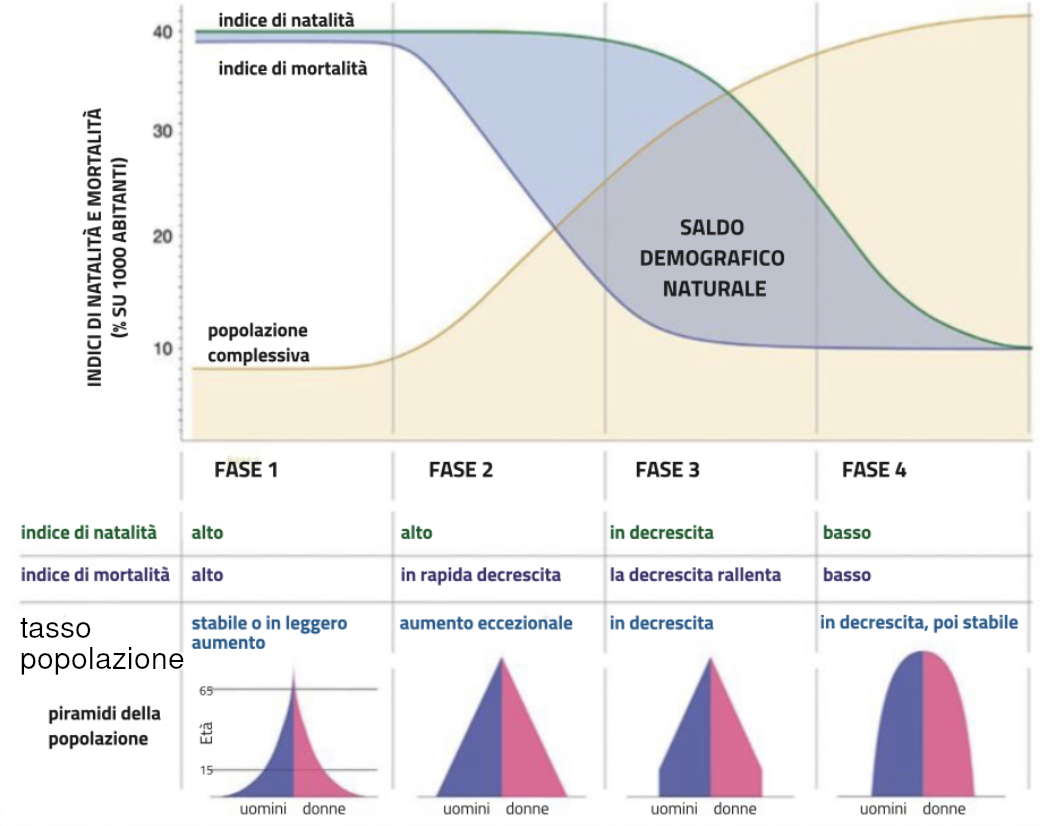
\includegraphics[width=\textwidth]{./resources/fasi_demografia.png}
    \end{figure}
    \end{center}
\end{snippet}

\end{document}